\chapter{Liste der gesichteten Urkunden}
\label{sec:urkliste}

Die folgenden zwei Listen enthalten die Urkundennummern im \tit{Corpus der
altdeutschen Originalurkunden} (\CAO), die für die Auswertung gesichtet wurden.
Dabei sind nicht sämtliche Urkunden in die Auswertung eingeflossen, da nicht
alle Belege für das untersuchte Phänomen enthalten. Überschneidungen mit dem
\REM{} und der \tit{Mittelhochdeutschen Grammatik} von \citet{ksw3,ksw2} sind
durch Kursivierung gekennzeichnet.

\section{Ausgewertete Urkunden}
\label{subsec:ausgewurk}

Die hier aufgelisteten Urkundennummern sind in die Stichprobe zur Auswertung von
\norm{bėide} `beide' eingeflossen, da sie relevante Belegstellen enthielten.

{%
\setlength{\columnsep}{35pt} % Aus langscibook.cls geschlossen (\p@ = 1.0 pt)
\raggedright
\begin{multicols}{2}
\begin{description}[font=\normalfont,labelsep=\fontdimen2\font]
\item[\cite{cao1},] 31, \emph{75}, \emph{76}, 81, \emph{85}, 86, 165, 171, 179,
190, 199, 201, 214, 260, 326, 371, 389, 415, \emph{429}, 491, \emph{508}, 519,
524, \emph{560}

\item[\cite{cao2},] 583, 604, 610, 619, 627, 629, 632, 636, 656, 682, 701, 923,
925, 937, 971~A, 971~B, 1001, 1055, 1073, 1121, 1126~A, 1126~B, 1137, 1153,
1154, 1201~A, 1201~B, 1217, 1218, 1221, 1229, 1234, 1259, 1270, 1282, 1352,
1359, 1382, 1414, 1416, 1436, 1503, 1504, 1514, 1545, 1566, 1568, 1578, 1584,
1620, 1657

\item[\cite{cao3},] 1661, 1747, 1764, 1802, 1831, 1843, 1898, 1950, 1956, 1971,
1972~A, 1972~B, \emph{2001}, 2011, 2055, 2092, 2110, 2174, 2183, 2214, 2240,
2253, 2293, 2307, 2309, 2310, 2338~A, 2338~B, 2350, 2353, 2359, 2367, 2375,
2396, 2401, 2406, 2412, 2445, 2468, 2497, 2532, 2535

\item[\cite{cao4},] 2563, 2568, 2583, 2625~A, 2625~B, 2651~A, 2651~B, 2694, 2713,
2719, \emph{2733} 2735~A, 2735~B, 2748, 2824, 2843, 2862, 2866, 2872, 2913,
2915, 2925, 2930, 2931, 2957, 2960, 2962, 3020~A, 3020~B, 3022, 3034, 3038,
3049, 3056, 3062, 3104, 3116, 3130, 3133, 3141~A, 3141~B, 3147, 3150, 3160,
3171, 3224~A, 3224~B, 3249, 3261, 3262, 3319, 3330, 3331, 3332, 3339, 3346,
3376, 3397, 3428, 3451, 3536

\item[\cite{cao5},] N~2~A, N~2~B, N~11, N~14, N~52, N~92, N~99, N~109~A,
N~109~B, N~150, N~197, N~202, N~210, N~220, N~230, N~235, \emph{N~272}, N~288,
N~294, N~305, N~321, N~328, N~357, N~377, N~384, N~385, N~386, N~401, N~456,
N~463, N~475, N~518, N~524, N~557, N~590, N~689, N~701, N~709, N~723, N~727,
N~748, N~752, N~756, N~766, N~812
\end{description}
\end{multicols}
}

\section{Ausgesonderte Urkunden}
\label{subsec:ausgesurk}

Neben solchen Urkunden, die im Ortsregister von \citet{cao-online} mehreren
Ausstellungsorten zugewiesen sind und/oder deren Ausstellungsjahr nicht
eindeutig feststellbar ist, wurden die im Folgenden aufgelisteten
Urkundennummern zusätzlich nicht in die Auswertung aufgenommen.

{%
\setlength{\columnsep}{35pt} % Aus langscibook.cls geschlossen (\p@ = 1.0 pt)
\raggedright
\begin{multicols}{2}
\begin{description}[font=\normalfont,labelsep=\fontdimen2\font]
\item[\cite{cao1},] 69~A, 71, \emph{72~B}, \emph{78}, \emph{83}, 131, 190, 369,
491, 501~A, 501~B, \emph{508}, \emph{549}, 559

\item[\cite{cao2},] 602, 623, 661~A, 661~B, \emph{677}, 777, 885, 904, 979,
1076, 1145, 1169, 1234, 1304, 1429, 1460

\item[\cite{cao3},] 1662, 1717, 1758, 1820, 1923, 2005, \emph{2008}, 2033, 2111,
2226, 2366, 2520, 2522, 2529

\item[\cite{cao4},] 2607, 2694, 2748, 2786, 2841, 3045, 3047, 3248, 3330, 3376,
3496

\item[\cite{cao5},] \emph{N~36}, \emph{N~68}, N~100, N~115, N~235, N~241, N~294,
N~305, N~337, N~524, N~526, N~567, N~664, N~674, N~702
\end{description}
\end{multicols}
}

%%%%%%%%%%%%%%%%%%%%%%%%%%%%%%%%%%%%%%%%%%%%%%%%%%%%%%%%%%%%%%%%%%%%%%%%%%%%%%%%

\chapter{Stichprobe zur Grafie von mhd.\ \norm{e}}
\label{sec:caoalemschwa}

Die Schreibweise \lit{i} für den unbetonten Nebensilbenvokal mittelhochdeutsch
\norm{e} [ə] gilt unter den ober\-deutschen Schreibdialekten als alemannisches
Kennzeichen \autocites[vgl.][25]{weinhold1863}[75]{weinhold1883}[41,
113]{paul2007}, jedoch findet sich \lit{-i} in der Stichprobe zu \norm{bėide}
`beide' typischerweise in solchen Kontexten, in denen ursprünglich \norm{-iu}
/yː/ vorlag. Um sicherzustellen, dass \lit{-i} in alemannischen Urkunden
tatsächlich die ebenfalls für diese Region typische Entrundung von \norm{-iu}
darstellt und nicht etwa regelmäßig auch an anderen Stellen für einen
unbetonten Vokal steht
\autocites%
	[466--467]{schirmunski1962}%
	[41]{paul2007}%
	[305]{ksw2}%
	[vgl.~auch][131--132]{boesch1946}%
, wurde eine gesonderte Teilauswertung auf Basis einer Stichprobe vorgenommen,
bei der die Grafie des Schwa-Lauts überprüft wurde.

Hierzu wurden die in \tabref{tab:caoalemschwa} aufgeführten Lemmata für die
Ausstellungsorte
Straßburg (2.600 Belege),
% 	āne		 254
% 	hērre	1832
% 	hȫrent	  27
% 	umbe	 367
% 	vrouwe	 120
% 	Summe	2600
% 
Zürich (1.695),
% 	āne		  63
% 	hērre	1121
% 	hȫrent	 144
% 	umbe	 254
% 	vrouwe	 113
% 	Summe	1695
% 
Freiburg i.\,Br. (1.478),
% 	āne		  95
% 	hērre	 865
% 	hȫrent	 160
% 	umbe	 226
% 	vrouwe	 132
% 	Summe	1478
% 
Basel (1.028),
% 	āne		  32
% 	hērre	 532
% 	hȫrent	 126
% 	umbe	 194
% 	vrouwe	 144
% 	Summe	1028
% 
Colmar (849),
% 	āne		 60
% 	hērre	393
% 	hȫrent	 93
% 	umbe	184
% 	vrouwe	119
% 	Summe	849
% 
Konstanz (1.110),
% 	āne		 110
% 	hērre	 657
% 	hȫrent	  93
% 	umbe	 207
% 	vrouwe	  43
% 	Summe	1110
% 
Luzern (236),
% 	āne		  8
% 	hērre	142
% 	hȫrent	 21
% 	umbe	 37
% 	vrouwe	 28
% 	Summe	236
% 
Bern (35)
% 	āne		 2
% 	hērre	13
% 	hȫrent	 6
% 	umbe	14
% 	vrouwe	 0
% 	Summe	35
% 
und Chur (45)
% 	āne		 2
% 	hērre	30
% 	hȫrent	 4
% 	umbe	 9
% 	vrouwe	 0
% 	Summe	45
% 
basierend auf der automatischen Annotation der Lemmata nach dem Modell von
\citet{schmid2019} abgefragt. Wie in \sectref{subsec:cao_sample} betreffend den
Aufbau der Stichprobe zur Adjektivdeklination im \tit{Corpus der altdeutschen
Originalurkunden} (\CAO) beschrieben, wurden auch hier jeweils die
Ausstellungsorte im Umkreis von etwa vierzig Kilometern (0,25°) hinzugenommen.
Die Lemmata wurden so ausgewählt, dass jeder im Ahd.\ volle Nebensilbenvokal
zumindest in der Zitationsform vorkommt und die Lemmata möglichst häufig im
\CAO{} belegt sind. Bei der Abfrage wurden nur solche Lemmata gewertet, deren
Zuweisung und Formenbestimmung der Annotations\-algorithmus mit mindestens
95\,\% Konfidenz bewertet hat.

\begin{table}
\setlength{\tabcolsep}{3.5pt}
\caption{Lemmata der Stichprobe zur Schwa-Grafie}
\begin{tabular}{l l l r r @{~} r l}
\lsptoprule

\mr{2}{*}[-.5ex]{Ahd.}
	& \mr{2}{*}[-.5ex]{Mhd.}
	& \mr{2}{*}[-.5ex]{Übersetzung}
	& \mc{3}{c}{Häufigkeit}
	& \mr{2}{*}[-.5ex]{Quelle}
	\\

\cmidrule(lr){4-6}

%
	& %
	& %
	& Stichprobe
	& %
	& \CAO{}
	& %
	\\

\midrule

\norm{hērro}
	& \norm{hērre}
	& `Herr'
	& 5.521
	& ca.
	& 17.700
	& \cite[834--837]{wmu1}
	\\

\norm{umbi}
	& \norm{umbe}
	& `um'
	& 1.482
	& ca.
	& 5.500
	& \cite[1857--1860]{wmu3}
	\\

\norm{frouwa}
	& \norm{vrouwe}
	& `(Edel-)Frau'
	& 688
	& ca.
	& 4.500
	& \cite[2261--2263]{wmu3}
	\\

\norm{hōrėnt}
	& \norm{hȫrent}
	& `(sie) hören'
	& 660
	& \norm{hȫren}:
	& 4.370
	& \cite[882--883]{wmu2}
	\\

\norm{ānu}
	& \norm{āne}
	& `ohne'
	& 621
	& %
	& 4.270
	& \cite[90--91]{wmu1}
	\\

\lspbottomrule
\end{tabular}
\label{tab:caoalemschwa}
\end{table}

Die Karte in \figref{fig:caoalemschwa} gibt einen Überblick über die geografische
Variation der Grafie des unbetonten Vokals in der Stichprobe. Gut zu sehen ist,
dass \norm{e} und die Syn- oder Apokope des Vokals -- wie beispielsweise bei
\lit{hern} `Herrn' und \lit{hoͤrnt} `hören (\textsc{3pl.ind.prs})' sowie
\lit{fron} `Frau (\textsc{obl.sg}), Frauen' und \lit{vmb} `um' -- vorherrschen.
Schreibungen mit anderen Vokalen kommen nur selten vor, zum Beispiel
\lit{herrun} `Herrn, Herren' oder \norm{frowan} `Frauen' (ahd. \norm{frouwūn}).
Darüber hinaus liegen noch einige Fälle von \lit{frown} vor, bei denen der
Nebensilbenvokal vermutlich synkopiert ist, jedoch die Schreibung \lit{w} für
\norm{wu} nicht strikt ausgeschlossen werden kann
\autocite[vgl.][142]{paul2007}. Ein großer prozentualer Anteil von Grafien mit
\norm{i} fällt besonders in St.~Gallen ins Auge.

\begin{figure}
\centering
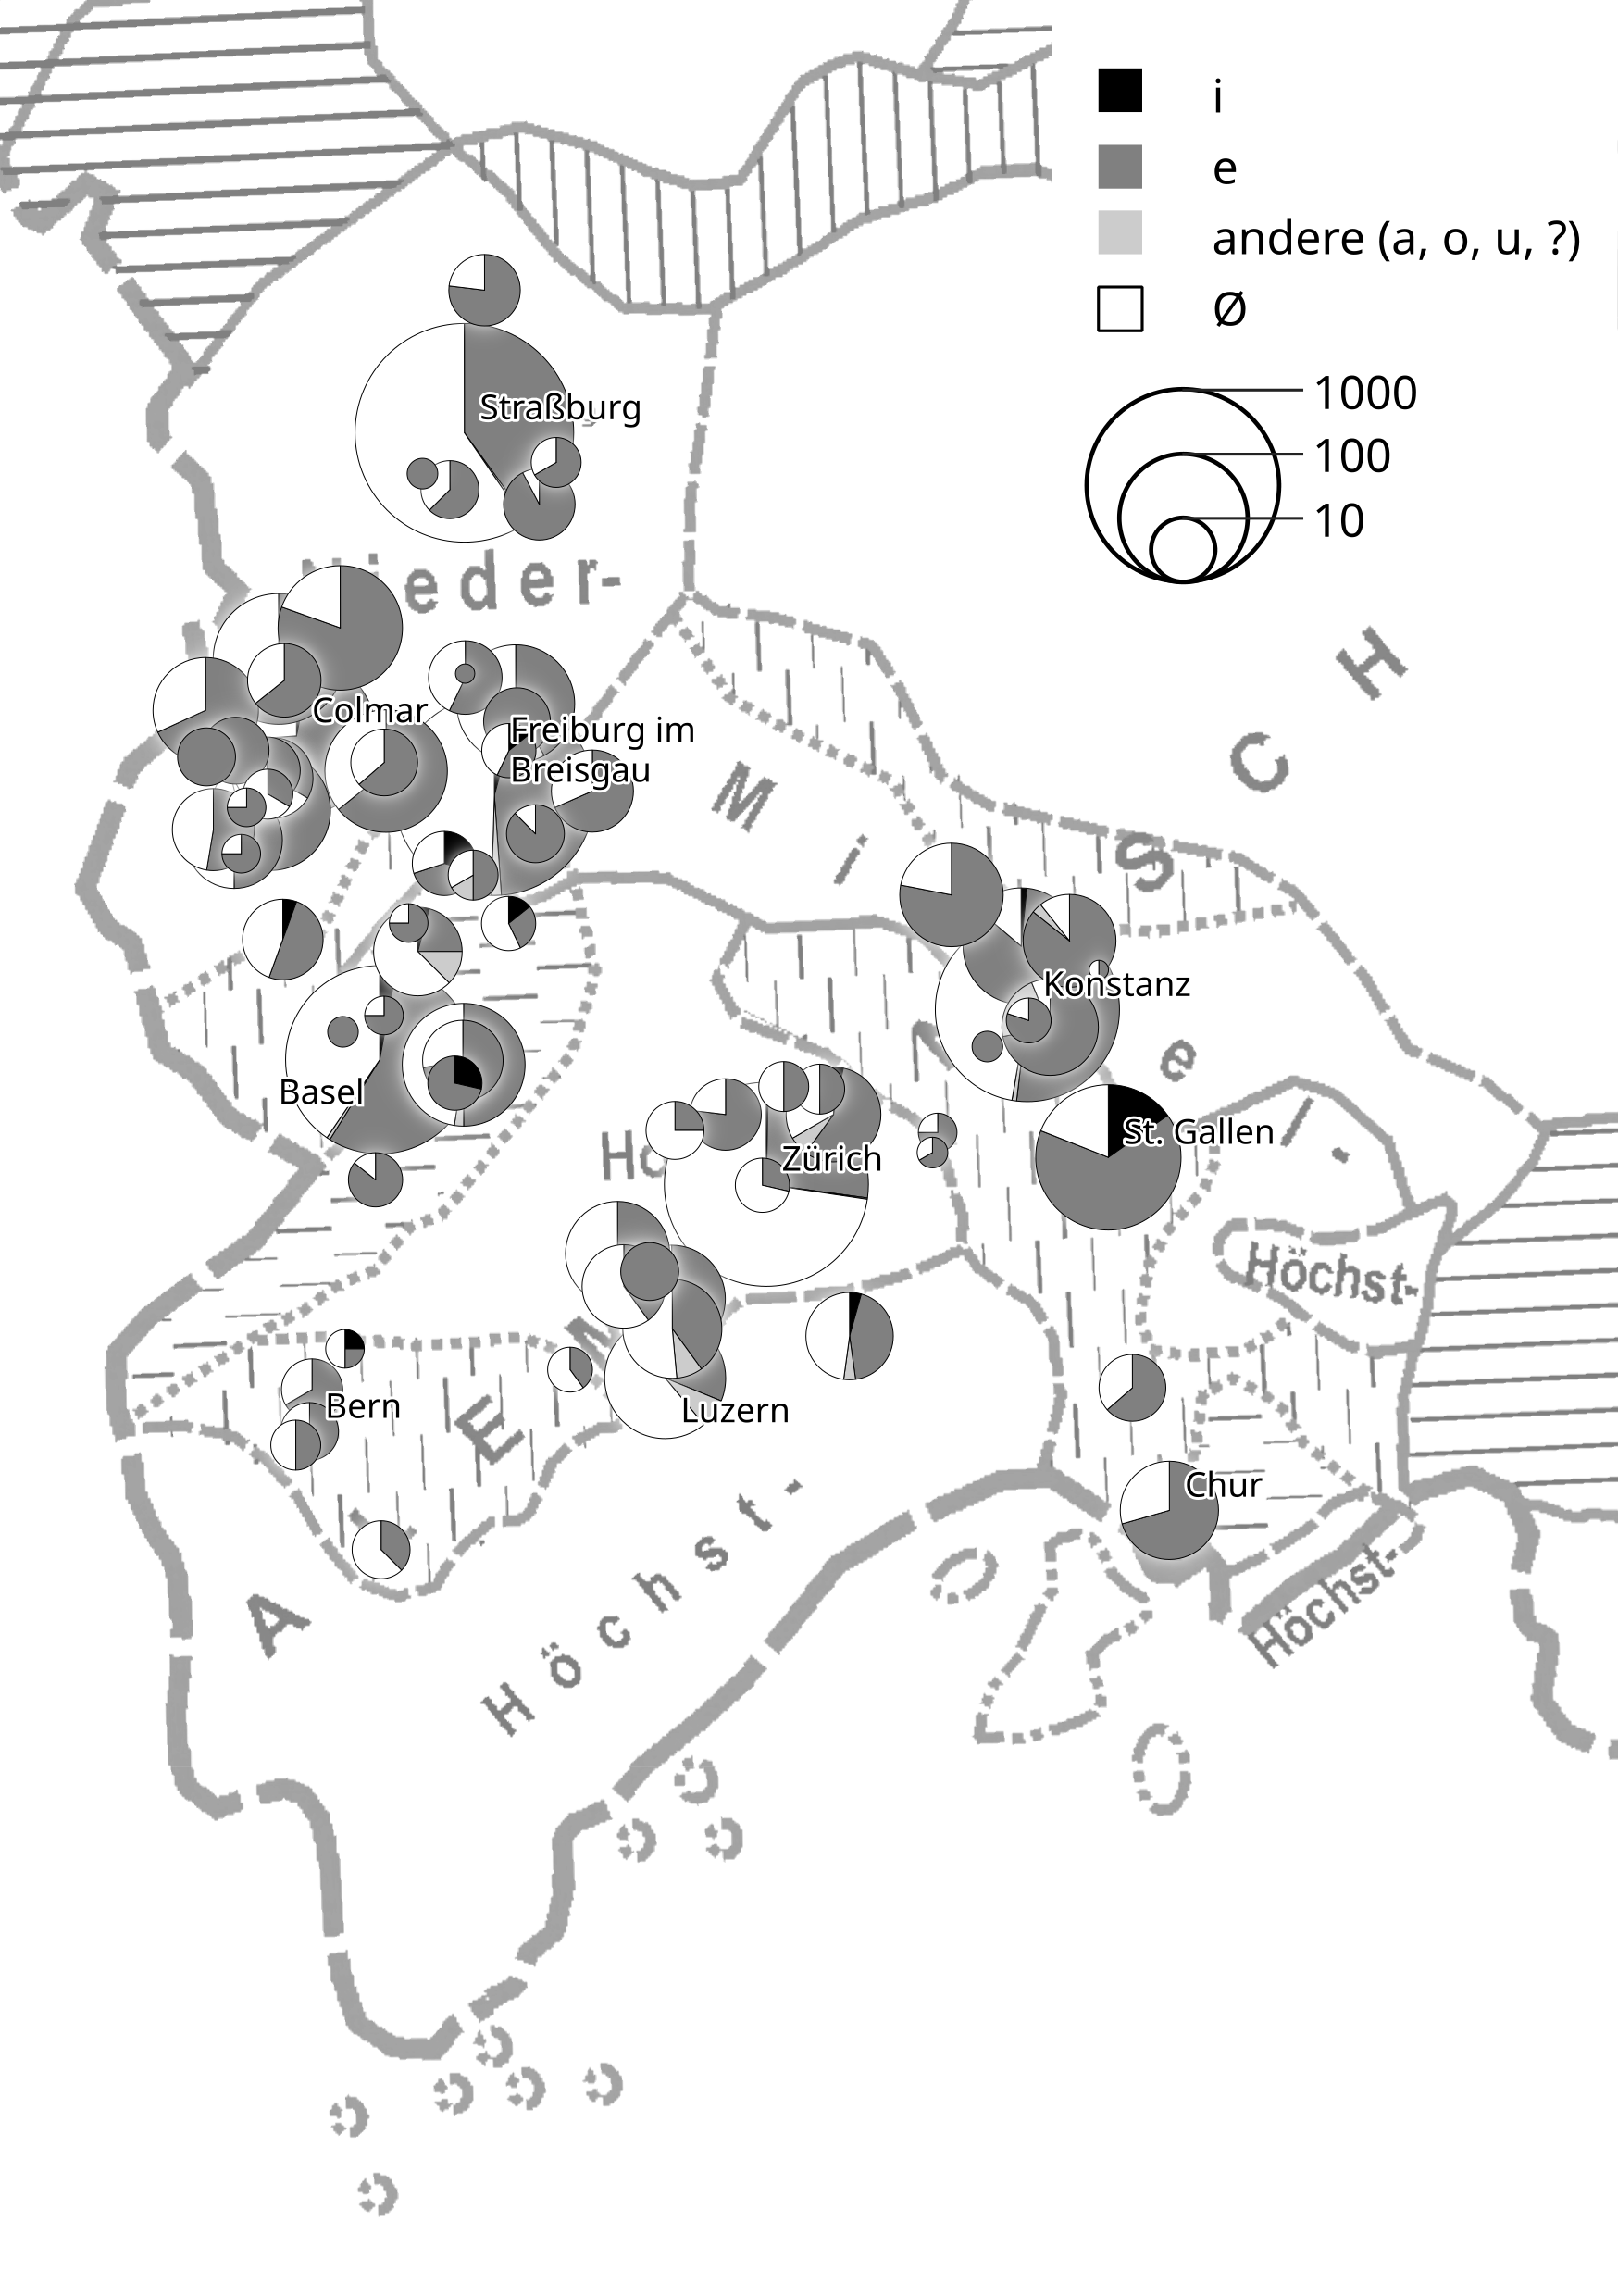
\includegraphics[
	width=\linewidth,
	height=\textheight,
	keepaspectratio
]{./figures/2023-05-19_schwa_alem.png}
\caption{Geografische Verteilung der Stichprobe zur Schwa-Grafie
(Hintergrundkarte: \cite{wiesinger1983:rede})}
\label{fig:caoalemschwa}
\end{figure}

In der Tat machen die 28 Belege aus St.~Gallen dort immerhin 15,2\,\% der
belegten \lit{i}-Grafien aus, wie aus \tabref{tab:ispelx} hervorgeht (diese zeigt
als Ausschnitt nur diejenigen Ausstellungsorte, an denen \norm{i}-Grafien
belegt sind). Hohe absolute Werte werden auch in Freiburg i.\,Br. (55 Belege)
sowie in Basel (25) und Konstanz (21) erreicht. Gemessen an der jeweiligen
Gesamtzahl der Belege pro Ausstellungsort machen sie allerdings nur einen
kleinen Teil aus (4,2\,\%; 2,9\,\%; 2,8\,\%). An anderen Ausstellungsorten in
der Stichprobe kommen \norm{i}-Grafien nur vereinzelt vor.

\begin{sidewaystable}
\caption{Varianten der Schwa-Grafie pro Schreibort}
\begin{tabular}{
	l @{\qquad}
	r r @{\qquad}
	r r @{\qquad}
	r r @{\qquad}
	r r @{\qquad}
	r}

\lsptoprule

Ausstellungsort
	& \norm{-i} & \%
	& \norm{-e} & \%
	& -Ø & \%
	& andere & \%
	& Summe
	\\

\midrule

Basel
	& 25	& 2,9
	& 481	& 56,0
	& 348	& 40,5
	& 5		& 0,6
	& 859
	\\

Colmar
	& 10	& 3,2
	& 222	& 70,7
	& 82	& 26,1
	& 		&
	& 314
	\\

Denzlingen
	& 1 & 14,3
	& 3	& 42,9
	& 3	& 42,9
	& 	&
	& 7
	\\

Freiburg i.\,Br.
	& 55	& 4,2
	& 589	& 44,7
	& 652	& 49,5
	& 21	& 1,6
	& 1317
	\\

Guebwiller
	& 1		& 3,1
	& 15	& 46,9
	& 16	& 50,0
	& 		&
	& 32
	\\

Kl.~Einsiedeln
	& 1		& 4,3
	& 10	& 43,5
	& 11	& 47,8
	& 1		& 4,3
	& 23
	\\

Kl.~Fraubrunnen
	& 1	& 25,0
	& 1	& 25,0
	& 2	& 50,0
	&	&
	& 4
	\\

Kl.~Olsberg
	& 2	& 28,6
	& 5	& 71,4
	&	&
	&	&
	& 7
	\\

Kl.~Sitzenkirch
	& 1		& 4,2
	& 5		& 20,8
	& 15	& 62,5
	& 3		& 12,5
	& 24
	\\

Kl.~Töss
	& 1		& 3,3
	& 17	& 56,7
	& 10	& 33,3
	& 2		& 6,7
	& 30
	\\

Konstanz
	& 21 	& 2,8
	& 364	& 49,1
	& 351	& 47,3
	& 6		& 0,8
	& 742
	\\

Luzern
	& 2		& 2,6
	& 22	& 28,6
	& 47	& 61,0
	& 6		& 7,8
	& 77
	\\

Mulhouse
	& 1	& 5,6
	& 9	& 50,0
	& 8	& 44,4
	&	&
	& 18
	\\

Schönau i.\,Sw.
	& 1	& 14,3
	& 2	& 28,6
	& 4	& 57,1
	&	&
	& 7
	\\

St.~Gallen
	& 28	& 15,2
	& 121	& 65,8
	& 35	& 19,0
	&		&
	& 184
	\\

Staufen i.\,Br.
	& 3 & 30,0
	& 4	& 40,0
	& 3	& 30,0
	&	&
	& 10
	\\

Überlingen
	& 1		& 1,5	
	& 55	& 84,6
	& 9		& 13,8
	&		&
	& 65
	\\

Zürich
	& 5		& 0,3
	& 406	& 26,8
	& 1100	& 72,7
	& 3		& 0,2
	& 1514
	\\

\lspbottomrule
\end{tabular}
\label{tab:ispelx}
\end{sidewaystable}

Die Form \lit{ani} für mhd.~\norm{āne}, ahd.~\norm{ānu} `ohne' ist ein einziges
Mal in Konstanz belegt und mit ihrem Kontext in \REF{ex:konst_ani} aufgeführt.

\begin{exe}
\ex\label{ex:konst_ani}
	\gll alſo daz ſie deſ gæltiſ gewiſſet vnde gwert werden ani giværde \\
		also dass sie des Geldes versichert und gewährt werden ohne
			Hinterhalt \\
	\trans `auf die Weise, dass sie ohne Arglist das Geld zugesichert und
		ausgezahlt bekommen'
		\parencites(Nr.~17, Konstanz, 1251)[26,22]{cao1}
\end{exe}

Auch \lit{umbi} `um', das zur Präposition mhd.~\norm{umbe}, ahd.~\norm{umbi}
gehört, tritt mit 4 Belegen nur selten in der Stichprobe auf. Es entfallen 3
Belege auf Colmar, zwei davon auf Nr.~N~53 \autocites(Colmar,
1264)[37,2--17]{cao5}, und 1 Beleg auf Freiburg i.\,Br. \autocites(Nr.~2580,
Freiburg i.\,Br., 1297)[9,21--33]{cao4}. Einer der Belege aus Colmar wird in
\REF{ex:col_umbi} zitiert.

\begin{exe}
\ex\label{ex:col_umbi}
	\gll daz wir {daz ſelbe} gvͦt vmbi daz halbe wider enpfangen han \\
		dass wir dasselbe Gut um das halbe wieder empfangen haben \\
	\trans `dass wir dasselbe Gut für die Hälfte \textins{der Einkünfte;
		vgl.~\cite[23]{caor}} zurückempfangen haben'
		\parencites(Nr.~N~92, Colmar, 1269)[64,27--28]{cao5}
\end{exe}

Bemerkenswert ist, dass in der Freiburger Urkunde Nr.~2590
\autocite[15,32--16,4]{cao4} außer dem einen Beleg für \lit{vmbi} `um'
(Z.~15,39) an allen sechs anderen Stellen die Form \lit{vmbe} steht und \lit{i}
auch sonst nicht als Grafie für Schwa dient.

Ähnlich schwach bezeugt sind Formen des Typs \lit{frowin} zu
mhd.~\norm{vrouwen} `Frau (\textsc{obl.sg}), Frauen', die sich auf 3 Belege aus
Colmarer und 2 aus Baseler Urkunden verteilen. Wie zu erwarten, stehen diese
Belege im Dat./Gen.~Sg. sowie im Nom.\ und Dat.~Pl., der im Ahd.\ in allen
Fällen \norm{frouwūn} lautete. Ein Beispiel wird in \REF{ex:col_vrouwin}
gegeben. Die Form kommt allein in dieser Urkunde noch zwei weitere Male vor,
was allen Colmarer Belegen entspricht. Über alle Ausstellungsorte in der
Stichprobe hinweg endet der Nom.~Sg.\ des Lemmas \norm{vrouwe} `(Edel-)Frau' in
64,6\,\% der Fälle auf \lit{-e}, in 31,5\,\% auf Ø und in lediglich 3,9\,\% auf
\lit{-a} (vgl.~ahd.~\norm{frouwa}), jedoch nie auf \norm{-i}.

\begin{exe}
\ex\label{ex:col_vrouwin}
	\gll {da mitte} die vorgenantin frowin geirrit / vnd biſwert moͤhtint
			werdin \\
		womit die vorgenannten Frau-\textsc{nom.pl.\FemF} gestört {} und
			belästigt könnten werden \\
	\trans `womit die vorgenannten Frauen gestört und belästigt werden
		könnten'
		\parencites(Nr.~3293, Colmar, 1299)[446,24]{cao4}
\end{exe}

Die Form \lit{herrin}, mhd.~\norm{hērren} `Herrn, Herren', die zurückgeht auf
ahd.~\norm{hērron, -un} (Akk.~Sg.\ und im Pl.) beziehungsweise
\norm{hērrin} (Gen./Dat.~Sg; \cite[vgl.][282--283]{braune2018}), ist in der
Stichprobe mit 43 Belegen vertreten, nämlich in St.~Gallen (12 Belege), Basel
(11), Freiburg i.\,Br. (5), Zürich (3), Colmar (2), Konstanz und Staufen
i.\,Br. (je 2) sowie in Guebwiller, Kl.~Olsberg, Kl.~Töss und Mulhouse (je 1).
Auffällig ist, dass allein 6 Belege für St.~Gallen auf die Urkunde Nr.~628
\autocite[55,35--57,7]{cao2} entfallen, aus der in \REF{ex:stg_herrin} zitiert
wird. Daneben tritt noch je einmal \lit{herri} zu mhd.~\norm{hērre},
ahd.~\norm{hērro} `Herr', in Colmar und Überlingen auf, wie in
\REF{ex:col_herri} gezeigt. Darüber hinaus steht in der gesamten Stichprobe in
87,4\,\% der Fälle im Nom.~Sg.\ eine Form vom Typ \lit{her}. Der Typ
\lit{herre} kommt mit 12,5\,\% wesentlich seltener vor, während sich die zwei
Fälle mit \lit{-i} auf lediglich 0,05\,\% belaufen. Formen wie *\lit{herro}
und *\lit{herru} sind in der Stichprobe nicht belegt.

\begin{exe}
\ex \label{ex:herrin}
	\begin{xlist}
	\ex\label{ex:stg_herrin}
		\setlength{\glossglue}{5pt plus 2pt minus 1pt}
		\gll dc denne die tohtira alle zemime herrin dim abte zeſant GAllin
				koment\\
			dass dann die Töchter alle zu=meinem Herr-\textsc{obl.sg.\MascM}
				dem Abt zu=Sankt Gallen kommen \\
		\trans `dass dann die Töchter alle zu meinem Herrn, dem Abt von
			St.~Gallen, kommen'
			\parencites(Nr.~628, St.~Gallen, 1284)[56,34]{cao2}

	\ex\label{ex:col_herri}
		\gll Do dirri brief geſcriben wart, do was vnſer herri dvſint vn̄ zwei
				hvndert vn̄ ſehzzit vn̄ vier iaric \\
			Als dieser Urkunde geschrieben wurde da war unser
				Herr-\textsc{nom.sg.\MascM} tausend und zwei hundert und
				sechzig und vier jährig \\
		\trans `Als diese Urkunde geschrieben wurde, da war unser Herr
			1.264 Jahre alt.'
			\parencites(Nr.~N~53, Colmar, 1264)[37,15]{cao5}
\end{xlist}
\end{exe}

Der größte Anteil an \lit{i}-Grafien in der Stichprobe entfällt auf Formen vom
Typ \lit{hörint} zu mhd.~\norm{hȫrent}, ahd.~\norm{hōrėnt} `hören
(\textsc{3pl.ind.prs})'. Die Belege verteilen sich auf die Ausstellungsorte
Freiburg i.\,Br. (43 Belege), Konstanz (18), St.~Gallen (15), Basel (12),
Zürich (2), Colmar, Denzlingen, Kl.~Einsiedeln, Kl.~Fraubrunnen, Kl.~Olsberg,
Kl.~Sitzenkirch, Luzern, Schönau i.\,Sw. und Staufen i.\,Br. (je 1). Hier
entfallen von den Belegen aus St.~Gallen 6 auf die Urkunde Nr.~629
\autocites(St.~Gallen, 1284)[57,9--57,35]{cao2}. Die Wortform \norm{hȫrent}
kommt stereotyp in der Promulgatio, also der Verkündigungsformel nahezu aller
Urkunden im \tit{Corpus} vor, wie in \REF{ex:fribr_hoerint} exemplarisch
angeführt.

\begin{exe}
\ex\label{ex:fribr_hoerint}
	\gll Allen die diſen brief ſehint oder hoͤrint leſin den kv̓nde ich fro
			Jvnte hern Cvͦnrat ſchnewelins ſeligen hvſfrôwe deſ jvngen von
			Friburch \\
		Allen die diesen Urkunde sehen-\textsc{3pl.ind.prs} oder
			hören-\textsc{3pl.ind.prs} lesen denen verkünde ich Frau Junte Herrn
			Konrad Schnewelins selige Ehefrau des Jungen von Freiburg \\
	\trans `Allen, die diese Urkunde sehen oder verlesen hören, verkünde
		ich, Frau Junte, die Ehefrau Herrn Konrads des Jungen von Freiburg
		selig \textelp{}'
		\parencites(Nr.~328, Freiburg i.\,Br., 1277)[314,33--34]{cao1}
\end{exe}

Insgesamt betrachtet kommt \lit{i} in der Stichprobe zwar als Schreibweise für
einen unbetonten Nebensilbenvokal vor, liegt aber in der Häufigkeit weit hinter
Schreibweisen mit \lit{e} zurück. Auffällig ist, dass \lit{i} in der Stichprobe
passend zu \posscite[132, 136--137]{boesch1946} Beobachtung nahezu
ausschließlich in gedeckten Nebensilben auftritt, also in unbetonter Stellung
vor Konsonant: \lit{herr\emph{in}}, \lit{frow\emph{in}}, \lit{hör\emph{in}t}.
Darüber hinaus zeigt gerade \lit{herrin} `Herren, Herrn' als schwaches
Maskulinum, dass \lit{i} an diesen Stellen unabhängig vom Lautwert der
entsprechenden Kasusform im Althochdeutschen steht
\autocite[vgl.][282--283]{braune2018}. Umgekehrt darf also davon ausgegangen
werden, dass Formen vom Typ \lit{beidi} `beide' nicht typischerweise
\lit{-i} für Schwa enthalten, zumal in keiner der betroffenen Urkunden
(\cites(Nrn.~81, 190)[124,18--33; 205,30--45]{cao1};
\cites(Nr.~N~230)[175,1--33]{cao5}) regelmäßig \lit{-i} im unbetonten absoluten
Auslaut steht.

%%%%%%%%%%%%%%%%%%%%%%%%%%%%%%%%%%%%%%%%%%%%%%%%%%%%%%%%%%%%%%%%%%%%%%%%%%%%%%%%

\chapter{Belegzahlen zur Adjektivstichprobe}
\label{sec:caoadjquanttab}

Die folgende Tabelle schlüsselt die Menge der ausgewerteten Belege pro
Ausstellungsort in der Stichprobe zur Adjektivflexion in \sectref{sec:adjdeclcao}
auf.

\section{Straßburg}

\begin{tabularx}{\linewidth}{X r r r r}
\lsptoprule
Ausstellungsort
	& \makecell{Urk.\\ insges.}
	& \makecell{Urk. in\\ Stichprobe}
	& \makecell{Belege\\ insges.}
	& \makecell{Belege\\ ausgew.}
	\\
\midrule

Straßburg
	& 219
	& 122
	& 408
	& 178
	\\

Appenweier
	& 1
	& 1
	& 7
	& 3
	\\

Haguenau
	& 3
	& 3
	& 10
	& 3
	\\

Kl. Eschau
	& 1
	& 1
	& 1
	& 1
	\\

\midrule

Summe
	& 224
	& 127
	& 426
	& 185
	\\

\lspbottomrule
\end{tabularx}

\section{Basel}

\begin{tabularx}{\linewidth}{X r r r r}
\lsptoprule
Ausstellungsort
	& \makecell{Urk.\\ insges.}
	& \makecell{Urk. in\\ Stichprobe}
	& \makecell{Belege\\ insges.}
	& \makecell{Belege\\ ausgew.}
	\\
\midrule

Basel
	& 117
	& 73
	& 216
	& 75
	\\

Beuggen
	& 4
	& 3
	& 9
	& 2
	\\

Mulhouse
	& 3
	& 3
	& 7
	& 2
	\\

Rheinfelden AG
	& 13
	& 12
	& 52
	& 14
	\\

\midrule

Summe
	& 137
	& 91
	& 284
	& 93
	\\

\lspbottomrule
\end{tabularx}

\section{Zürich}

\begin{tabularx}{\linewidth}{X r r r r}
\lsptoprule
Ausstellungsort
	& \makecell{Urk.\\ insges.}
	& \makecell{Urk. in\\ Stichprobe}
	& \makecell{Belege\\ insges.}
	& \makecell{Belege\\ ausgew.}
	\\
\midrule

Zürich
	& 143
	& 74
	& 244
	& 70
	\\

Eschenbach LU
	& 6
	& 6
	& 34
	& 9
	\\

Hohenrain
	& 8
	& 6
	& 31
	& 15
	\\

Kl. Einsiedeln
	& 3
	& 2
	& 8
	& 3
	\\

Kl. Töss
	& 6
	& 3
	& 16
	& 4
	\\

Regensberg
	& 3
	& 3
	& 5
	& 2
	\\

\midrule

Summe
	& 169
	& 94
	& 338
	& 103
	\\

\lspbottomrule
\end{tabularx}

\section{Konstanz}

\begin{tabularx}{\linewidth}{X r r r r}
\lsptoprule
Ausstellungsort
	& \makecell{Urk.\\ insges.}
	& \makecell{Urk. in\\ Stichprobe}
	& \makecell{Belege\\ insges.}
	& \makecell{Belege\\ ausgew.}
	\\
\midrule

Konstanz
	& 46
	& 36
	& 202
	& 55
	\\

Kl. Kreuzlingen
	& 1
	& 1
	& 6
	& 2
	\\

Kl. Münsterlingen
	& 4
	& 1
	& 14
	& 4
	\\

Kl. Salem
	& 5
	& 5
	& 13
	& 4
	\\

Nellenburg
	& 2
	& 2
	& 24
	& 7
	\\

Schloss Altenklingen
	& 1
	& 1
	& 2
	& 1
	\\

St. Gallen
	& 16
	& 15
	& 68
	& 22
	\\

Tannegg
	& 1
	& 1
	& 9
	& 2
	\\

Überlingen
	& 14
	& 9
	& 27
	& 10
	\\

\midrule

Summe
	& 92
	& 73
	& 370
	& 107
	\\

\lspbottomrule
\end{tabularx}

\section{Ulm}

\begin{tabularx}{\linewidth}{X r r r r}
\lsptoprule
Ausstellungsort
	& \makecell{Urk.\\ insges.}
	& \makecell{Urk. in\\ Stichprobe}
	& \makecell{Belege\\ insges.}
	& \makecell{Belege\\ ausgew.}
	\\
\midrule

Ulm
	& 16
	& 15
	& 64
	& 34
	\\

Kl. Blaubeuren
	& 1
	& 1
	& 9
	& 6
	\\

Kl. Herbrechtingen
	& 1
	& 1
	& 8
	& 5
	\\

\midrule

Summe
	& 18
	& 17
	& 81
	& 45
	\\

\lspbottomrule
\end{tabularx}

\section{Augsburg}

\begin{tabularx}{\linewidth}{X r r r r}
\lsptoprule
Ausstellungsort
	& \makecell{Urk.\\ insges.}
	& \makecell{Urk. in\\ Stichprobe}
	& \makecell{Belege\\ insges.}
	& \makecell{Belege\\ ausgew.}
	\\
\midrule

Augsburg
	& 95
	& 78
	& 517
	& 141
	\\

Adelzhausen
	& 1
	& 1
	& 6
	& 2
	\\

Aichach
	& 4
	& 3
	& 34
	& 14
	\\

Bocksberg (Laugna)
	& 1
	& 1
	& 13
	& 5
	\\

Kl. Holzen
	& 2
	& 2
	& 8
	& 4
	\\

Kl. Oberschönenfeld
	& 5
	& 5
	& 14
	& 2
	\\

Kl. Weihenberg
	& 1
	& 1
	& 1
	& 1
	\\

\midrule

Summe
	& 109
	& 91
	& 593
	& 169
	\\

\lspbottomrule
\end{tabularx}

\section{Nürnberg}

\begin{tabularx}{\linewidth}{X r r r r}
\lsptoprule
Ausstellungsort
	& \makecell{Urk.\\ insges.}
	& \makecell{Urk. in\\ Stichprobe}
	& \makecell{Belege\\ insges.}
	& \makecell{Belege\\ ausgew.}
	\\
\midrule

Nürnberg
	& 26
	& 18
	& 76
	& 39
	\\

Kl. Seligenporten
	& 3
	& 3
	& 44
	& 20
	\\

\midrule

Summe
	& 29
	& 21
	& 120
	& 59
	\\

\lspbottomrule
\end{tabularx}

\section{Regensburg}

\begin{tabularx}{\linewidth}{X r r r r}
\lsptoprule
Ausstellungsort
	& \makecell{Urk.\\ insges.}
	& \makecell{Urk. in\\ Stichprobe}
	& \makecell{Belege\\ insges.}
	& \makecell{Belege\\ ausgew.}
	\\
\midrule

Regensburg
	& 53
	& 43
	& 245
	& 88
	\\

Abensberg
	& 1
	& 1
	& 4
	& 2
	\\

Kl. Pettendorf
	& 5
	& 3
	& 17
	& 6
	\\

Kl. Pielenhofen
	& 5
	& 4
	& 16
	& 6
	\\

Laaber
	& 1
	& 1
	& 5
	& 3
	\\

\midrule

Summe
	& 65
	& 52
	& 287
	& 105
	\\

\lspbottomrule
\end{tabularx}

\section{München}

\begin{tabularx}{\linewidth}{X r r r r}
\lsptoprule
Ausstellungsort
	& \makecell{Urk.\\ insges.}
	& \makecell{Urk. in\\ Stichprobe}
	& \makecell{Belege\\ insges.}
	& \makecell{Belege\\ ausgew.}
	\\
\midrule

München
	& 22
	& 19
	& 94
	& 54
	\\

Kl. Indersdorf
	& 2
	& 2
	& 13
	& 6
	\\

Sachsenhausen (Egling)
	& 1
	& 1
	& 13
	& 6
	\\

\midrule

Summe
	& 25
	& 20
	& 120
	& 66
	\\

\lspbottomrule
\end{tabularx}

\section{Salzburg}

\begin{tabularx}{\linewidth}{X r r r r}
\lsptoprule
Ausstellungsort
	& \makecell{Urk.\\ insges.}
	& \makecell{Urk. in\\ Stichprobe}
	& \makecell{Belege\\ insges.}
	& \makecell{Belege\\ ausgew.}
	\\
\midrule

Salzburg
	& 75
	& 59
	& 309
	& 88
	\\

Burgstall Kalham
	& 1
	& 1
	& 4
	& 1
	\\

Kl. Berchtesgaden
	& 2
	& 1
	& 12
	& 3
	\\

Kl. Höglwörth
	& 1
	& 1
	& 2
	& 2
	\\

Kl. Michaelbeuern
	& 1
	& 1
	& 14
	& 3
	\\

Mattsee
	& 1
	& 1
	& 6
	& 2
	\\

Reichenhall
	& 2
	& 1
	& 2
	& 1
	\\

Schloss Staufeneck
	& 2
	& 2
	& 9
	& 2
	\\

\midrule

Summe
	& 85
	& 67
	& 358
	& 102
	\\

\lspbottomrule
\end{tabularx}

\section{Wien}

\begin{tabularx}{\linewidth}{X r r r r}
\lsptoprule
Ausstellungsort
	& \makecell{Urk.\\ insges.}
	& \makecell{Urk. in\\ Stichprobe}
	& \makecell{Belege\\ insges.}
	& \makecell{Belege\\ ausgew.}
	\\
\midrule

Wien
	& 51
	& 45
	& 197
	& 60
	\\

Kaiserebersdorf
	& 4
	& 2
	& 14
	& 6
	\\

Klosterneuburg
	& 9
	& 8
	& 45
	& 14
	\\

Stift Heiligenkreuz
	& 8
	& 8
	& 40
	& 12
	\\

\midrule

Summe
	& 71
	& 58
	& 296
	& 92
	\\

\lspbottomrule
\end{tabularx}

%%%%%%%%%%%%%%%%%%%%%%%%%%%%%%%%%%%%%%%%%%%%%%%%%%%%%%%%%%%%%%%%%%%%%%%%%%%%%%%%

\chapter{Verzeichnis der zitierten Handschriften}
\label{ch:hssverz}

Die folgenden Handschriftensignaturen werden im Text genannt. Weiterführende
Informationen zur jeweiligen Handschrift sowie Links zu Digitalisaten können
dem \tit{Handschriftencensus} (\tit{HSC}; \nosh\cite{hsc}) unter der
angegebenen ID entnommen werden, zum Beispiel
\url{https://handschriftencensus.de/1432} für A1. Weil es sich nicht in allen
Fällen um -- im weitesten Sinn -- literarische Texte oder deutsch\-sprachige
Werke handelt, existiert nicht zu jeder genannten Signatur ein Eintrag im
\tit{HSC}.\\

\noindent
\begin{tabularx}{\linewidth}{@{} >{\raggedright\arraybackslash}X l @{}}
Basel, Universitätsbibliothek, Cod. B VIII 27
	& \autocite[2776]{hsc} \\
Basel, Universitätsbibliothek, Cod. N I 3, Nr. 89
	& \autocite[1158]{hsc} \\
Bern, Staatsarchiv, StABE C I a, Stift 1293.11.30
	& --- \\
Dresden, Sächsische Landesbibliothek, Mscr.Dresd.M.32
	& \autocite[7549]{hsc} \\
Gießen, Universitätsbibliothek, Hs 97
	& \autocite[1102]{hsc} \\
Heidelberg, Universitätsbibliothek, Cod. Pal. germ. 361
	& \autocite[1181]{hsc} \\
Heidelberg, Universitätsbibliothek, Cod. Pal. germ. 848
	& \autocite[4957]{hsc} \\
Karlsruhe, Badische Landesbibliothek, Cod. Aug. 52
	& \autocite[8470]{hsc} \\
Köln, Historisches Archiv der Stadt, Best. 210 (Domstift), U~3/759
	& ---%
	% \footnote{Digitalisat: \url{https://historischesarchivkoeln.de/document/Vz_E9493491-3A61-4625-8DB0-09465C24BCC8}.}
	\\
Leutkirch, Fürstliche Waldburg zu Zeil und Trauch\-burg\-sches
	Gesamt\-archiv, ZAMs 30
	& \autocite[8471]{hsc} \\
München, Bayerische Staatsbibliothek, Cgm 25
	& \autocite[8827]{hsc} \\
München, Bayerische Staatsbibliothek, Cgm 37
	& \autocite[2119]{hsc} \\
München, Bayerische Staatsbibliothek, Cgm 44
	& \autocite[1307]{hsc} \\
München, Bayerische Staatsbibliothek, Cgm 51
	& \autocite[1286]{hsc} \\
München, Bayerische Staatsbibliothek, Cgm 183
	& \autocite[9715]{hsc} \\
München, Bayerische Staatsbibliothek, Cgm 965
	& \autocite[8472]{hsc} \\
München, Bayerische Staatsbibliothek, Cgm 6247
	& \autocite[1450]{hsc} \\
München, Bayerische Staatsbibliothek, Clm 16083
	& \autocite[19293]{hsc} \\
Nordhausen, Stadtarchiv, Ms. II, Na 6
	& \autocite[1379]{hsc} \\
Nürnberg, Germanisches Nationalmuseum, Hs. 22067
	& \autocite[1189]{hsc} \\
Oxford, Bodleian Lib., Cod. Junius 11
	& ---%
	% \footnote{Digitalisat: \url{https://digital.bodleian.ox.ac.uk/objects/d5e3a9fc-abaa-4649-ae48-be207ce8da15/}.}
	\\
\end{tabularx}

\noindent
\begin{tabularx}{\linewidth}{@{} >{\raggedright\arraybackslash}X l @{}}
Reykjavík, Stofnun Árna Magnússonar, GKS 2365 4to
	& ---%
	% \footnote{Digitalisat: \url{https://handrit.is/manuscript/view/is/GKS04-2365/31}.}
	\\
St. Gallen, Stiftsbibliothek, Cod. Sang. 857
	& \autocite[1211]{hsc} \\
Straßburg, Bibliothèque nationale et universitaire, ms. 2215
	& \autocite[1828]{hsc} \\
Prag, Národní knihovna České republiky, Cod. XIII.G.43
	& \autocite[1168]{hsc} \\
Uppsala, Universitätsbibliothek, MS DG 1
	& ---%
	% \footnote{Digitalisat: \url{http://www.alvin-portal.org/alvin/view.jsf?pid=alvin-record:60279}.}
	\\
Vorau, Archiv des Augustiner-Chorherrenstifts, Ms 276
	& \autocite[1432]{hsc} \\
Wien, Österreichische Nationalbibliothek, Cod. 2685
	& \autocite[2013]{hsc} \\
Wien, Österreichische Nationalbibliothek, Cod. 2687
	& \autocite[6494]{hsc} \\
Wien, Österreichische Nationalbibliothek, Cod. 2693
	& \autocite[1215]{hsc} \\
Wien, Österreichische Nationalbibliothek, Cod. 2779
	& \autocite[2693]{hsc} \\
Wien, Österreichische Nationalbibliothek, Cod. 12487
	& \autocite[3394]{hsc} \\
Wolfenbüttel, Herzog August Bibliothek, Cod. Guelf. 3.1 Aug. 2º
	& \autocite[8396]{hsc} \\
Wolfenbüttel, Herzog August Bibliothek, Cod. Guelf. 15.2 Aug. 2º
	& \autocite[6668]{hsc} \\
\end{tabularx}
